\documentclass{article}

\usepackage{geometry}
\usepackage[hidelinks, bookmarks = true]{hyperref}
\usepackage[numbered]{bookmark}
\usepackage{booktabs}
\usepackage{float}
\usepackage{graphicx}
\usepackage{geometry}
\usepackage{titletoc}
\usepackage{indentfirst}
\usepackage{fancyhdr} 
\usepackage{longtable}
\usepackage{supertabular}
\usepackage[normalem]{ulem}
\usepackage{listings}
\usepackage{xcolor}
\usepackage{xurl}
\usepackage{tikz}
\usepackage{lastpage}
\usepackage{amsmath}
\usepackage{amssymb}
\usepackage{mathtools}
\usepackage{caption}
\usepackage{threeparttable}
\usepackage{subcaption}

\geometry{a4paper, left = 1.9cm, right = 1.9cm, top = 2.3cm, bottom = 2.3cm, includehead}
\captionsetup[table]{font={small}}

\pagestyle{fancy}
\fancyhead[R]{\thepage /\pageref{LastPage}}
\fancyhead[L]{GROUP 28}
\fancyfoot{}
\fancyfoot{}
\renewcommand{\headrulewidth}{0pt}
\renewcommand{\footrulewidth}{0pt}
\setlength{\headheight}{14.49998pt}
\addtolength{\topmargin}{-2.49998pt}

\begin{document}
\noindent\rule{\textwidth}{1pt}
\begin{center}
    \LARGE \textbf{Assignment 1: Recommender Systems}
\end{center}
\noindent\rule{\textwidth}{0.5pt}
\begin{center}
    \textbf{Group 28}\par
    \vspace{0.3cm}
Shuang Fan\phantom{space}Kaiteng Jiang\phantom{space}Shupei Li\\
s3505847\phantom{spacespac}s3479420\phantom{spacespa}s3430863
\end{center}
\section{Recommender systems}
RMSE and MAE are chosen as metrics in Task 1.1-1.3. The predicted value in all task is a real number that may exceed the valid range of rating. To fix this problem, we truncate the predicted value according to the function,
\begin{align*}
    f(\hat{x}) &= 
    \begin{cases}
        1,\qquad &\hat{x} < 1,\\
        \hat{x},\qquad &1\leq \hat{x} \leq 5,\\
        5, \qquad &\hat{x} > 5.
    \end{cases}
\end{align*}
\par
It is worth noting that we set the random seed to 1 in all models that involve randomness, e.g. weights initialization, five-fold division, etc. The fixed random state ensures reproducibility.\par
When analyzing the complexity of the algorithm, we use the following notations.
\begin{itemize}
    \item $M$: The number of movies.
    \item $U$: The number of users.
    \item $R$: The number of ratings.
    \item $K$: The number of features.
\end{itemize}
In Task 1.2 and 1.3, the number of features $K$ is an integer specified by user. We regard $K$ as a constant in the algorithm analysis.\par

\subsection{Naive Approaches}
\subsubsection{Experimental Setup}
During the sampling process of an "average rating" recommender, some users or some movies might disappear from the training sets. To fix this problem, we need to define a fall-back value. In our experiments, we build models of global average, user average, movie average and a linear combination of user and movie averages (with and without the intercept). A linear regression model can be expressed as,
\begin{align*}
    pred&=\alpha\cdot avg_{user} + \beta\cdot avg_{movie} + \gamma,
\end{align*}
where $\gamma$ is the intercept. After simplifing the variant $\gamma$, we get,
\begin{align*}
    pred&=\alpha\cdot avg_{user} + \beta\cdot avg_{movie}.
\end{align*}
\par
Considering the matrix $\mathbf{U}$ with UserID and MovieID, the global average should be the average value of all existed Ratings. For user average rating, we calculate every user's average rating. This is the $avg_{user}$ term in the equation. For movie average rating, we calculate every movie's average rating. This is the $avg_{movie}$ term in the equation. When implementing the linear regression algorithm, we calculate the coefficient and consider the situations that are with and without the intercept $\gamma$.\par
All experiments of Task 1.1 are run on a multi-core CPU Intel(R) Core(TM) i9-9880H CPU @ 2.30GHz.
\subsubsection{Results}
Table \ref{tab:1.1-results} reports RMSE, MAE, and the actual run time of global average, user average, movies average and a linear combination of user and movie averages(with and without the intercept). RMSE and MAE are the mean values of five folds.
\begin{table}[ht]
    \centering
    \caption{Results of Task 1.1}
    \label{tab:1.1-results}
    \begin{threeparttable}
    \begin{tabular}{lllllllll}
        \toprule
        \textbf{Algorithm}  & \textbf{Train RMSE} & \textbf{Train MAE} & \textbf{Test RMSE} & \textbf{Test MAE} & \textbf{Time}\\
        \midrule
        GlobalAvg & 1.1171 & 0.9339 & 1.1171 & 0.9339 & 0.93s\\
        UserAvg & 1.0277 & 0.8227 & 1.0355 & 0.8290 & 1.38s\\
        MovieAvg & 0.9742 & 0.7783 & 0.9794 & 0.7823 & 1.43s\\
        LinearReg & \textbf{0.9145} & \textbf{0.7248} & \textbf{0.9002} & \textbf{0.7122} & 13m 57s\\
        LinearRegNI & 0.9465 & 0.7586 & 0.9345 & 0.7487 & 13m 45s\\
        \bottomrule
    \end{tabular}
    \end{threeparttable}
\end{table}

\subsubsection{Algorithm Analysis}
\noindent\textbf{Time Complexity}\\
In the model construction stage, computing the global average rating has the $O(R)$ time complexity, since the number of addition operations is $R - 1$ and the number of division operation is $1$. When calculating the average movie rating, we need  $O(R)$ addition operations and $O(M)$ division operations for all movies. Therefore, the time complexity of calculating the average movie rating is $O(M + R)$. Similarly, calculating the average user rating has the $O(U + R)$ time complexity. Linear regression can be written in the matrix form as follows.
$$
Y = X\beta
$$
where $X$ is an $I\times J$ matrix. Then, the result of linear regression is,
$$
\hat{\beta} = \left[ X^TX \right]^{-1} X^TY
$$
The time complexity of estimating $\beta$ is $O(I\times J^2 + J^3)$. $I$ equals to $R$ in Task 1.1. $J$ is $3$ if linear regression is with intercept term, and is $2$ if without intercept term. Thus, the time complexity of linear regression algorithm is $O(U + R) + O(M + R) + O(c^2R + c^3)\rightarrow O(U + M + R)$, where $c$ is a constant. In all five models, evaluating RMSE and MAE has the time complexity of $O(R)$. The following summarizes the time complexity of five models.
\begin{itemize}
    \item Global average rating: $O(R)$.
    \item Average movie rating: $O(M + R)$.
    \item Average user rating: $O(U + R)$.
    \item Linear regression (with and without intercept): $O(U + M + R)$.
\end{itemize}
\par
\vspace{0.3cm}
\noindent\textbf{Memory Complexity}\\
Storing all ratings needs $O(R)$ memory. When calculating the global average rating, we only need to maintain one number that is the average value. It means that calculating the global average rating has $O(R) + O(1)\rightarrow O(R)$ memory complexity. As for computing the average movie rating, we firstly needs to maintain an $M\times 1$ array. Then, we calculate the mean value of the array. Therefore, the memory complexity of computing the average movie rating is $O(R + M + 1) \rightarrow O(R + M)$. We can analyze the process of computing the average user rating similarly and obtain $O(R + U)$ complexity.
When adopting linear regression models, we needs an additional $O(1)$ memory to store $\beta$. Besides, calculating RMSE and MAE requires $O(R)$ memory in all five models. The memory complexity of five models is listed as follows.
\begin{itemize}
    \item Global average rating: $O(R)$.
    \item Average movie rating: $O(M + R)$.
    \item Average user rating: $O(U + R)$.
    \item Linear regression (with and without intercept): $O(U + M + R)$.
\end{itemize}

\subsection{UV Matrix Decomposition}
\subsubsection{Experimental Set-up}
The UV matrix decomposition is an element-wise update algorithm of the feature matrices $U_{m\times k}$ and $V_{k\times n}$, of which the multiplication $UV$ approximates the utility matrix $M_{m\times n}$. The goal of update is to minimize the mean square error (MSE) function. For an element $u_{rs}$ of the matrix $U$, the optimization problem can be written as,
\[
u_{rs} = \min_{x} \sum_{j, m_{rj}\neq 0}\left[ m_{rj}-\left( \sum_{k\neq s}u_{rk}v_{kj} + xv_{sj} \right) \right]^2.
\]
And for $v_{rs}$,
\[
v_{rs} = \min_{y} \sum_{i, m_{is}\neq 0}\left[ m_{is}-\left( \sum_{k\neq r}u_{ik}v_{ks} + u_{ir}y \right) \right]^2.
\]

They both have closed-form solutions,
\begin{align*}
x &= \frac{\sum\limits_{j, m_{rj}\neq 0}v_{sj}\left(m_{rj}-\sum\limits_{k\neq s }u_{rk}v_{kj}\right)}
{\sum\limits_{j, m_{rj}\neq 0}v_{sj}^2},\\
y &= \frac{\sum\limits_{i, m_{is}\neq 0}u_{ir}\left(m_{is}-\sum\limits_{k\neq s }u_{ik}v_{ks}\right)}
{\sum\limits_{i, m_{is}\neq 0}u_{ir}^2}. 
\end{align*}

In the experiment, we visit every element of both $U$ and $V$ in a random order per epoch. And predicted values are clipped to the range of $[1,5]$, as mentioned at the beginning of the section. Table \ref{tab:1.2-hyper} explains the hyperparameters in the algorithm.
\begin{table}[ht]
    \centering
    \caption{Hyperparameters in UV Matrix Factorization}
    \label{tab:1.2-hyper}
    \begin{tabular}{ll}
        \toprule
        \textbf{Hyperparameter} & \textbf{Meaning}\\
        \midrule
        seeds & The random seed. Default: 1.\\
        num\_factors ($K$) & The number of features.\\
        num\_iter ($N$) & The maximum iteration.\\
        \bottomrule
    \end{tabular}
\end{table}

\subsubsection{Results}
Table \ref{tab:1.2-re} reports the results of the task.
\begin{table}[ht]
    \centering
    \caption{Results of Task 1.2}
    \label{tab:1.2-re}
    \begin{tabular}{lllllll}
        \toprule
        \textbf{$K$} & \textbf{$N$} & \textbf{Train RMSE} & \textbf{Train MAE} & \textbf{Test RMSE} & \textbf{Test MAE} & \textbf{Time}\\
        \midrule
        5 & 30 & 0.8270 & 0.6486 & 0.8979 & 0.7005 & 72m 25s\\
        \bottomrule
    \end{tabular}
\end{table}

\subsubsection{Algorithm Analysis}
\noindent\textbf{Time Complexity}\\
Computing the sum $\sum_{k}$ needs time $O(K)$, and $\sum_j$ needs $O(M)$. Thus, a single update of an element of $U$ costs $O(MK)$. Similarly, updating an element of $V$ needs $O(UK)$. Since there are $UK$ and $KM$ elements in $U$ and $V$ respectively, an epoch which updates all the elements of $U$ and $V$ has a time complexity of $O(UK\cdot MK+KM\cdot UK)=O(MUK^2)\rightarrow O(MU)$. This is a very costly and slow algorithm, which explains the long running time in the experiment result. In fact, we have tried to set the dimension $K$ to larger numbers, like 10, and it took many hours to run a single experiment, which became unacceptable.

\vspace{0.3cm}
\noindent\textbf{Memory Complexity}\\
We only need to initialize, store and update three matrices: $U$, $V$ and $M$, thus the memory complexity is $O(UK+MK+R)\rightarrow O(U+M+R)$.

\subsection{Matrix Factorization}
\subsubsection{Experimental Set-up}
Matrix factorization algorithm in \texttt{gravity-Tikk.pdf} consists of three stages --- initialization, gradient descent, and evaluation. In the experiments, we initialize feature matrices $\mathbf{U}_{I\times K}$ and $\mathbf{M}_{K\times J}$ from a Gaussian distribution $N\sim (0, 0.1)$, where $I$, $J$, and $K$ are maximal UserID, maximal MovieID, and the number of features respectively. \texttt{gravity-Tikk.pdf} combines gradient descent and regularization strategies. Main update formulas are,
\begin{align*}
    u_{ik}^{(t+1)} &= u_{ik}^{(t)} + \eta\cdot\left( 2e_{ij}\cdot m_{kj}^{(t)} - \lambda\cdot u_{ik}^{(t)} \right) \\
    m_{kj}^{(t+1)} &= m_{kj}^{(t)} + \eta\cdot\left( 2e_{ij}\cdot u_{ik}^{(t)} - \lambda \cdot m_{kj}^{(t)} \right) 
\end{align*}
where $\eta$, $\lambda$ are hyperparameters, and $t$ represents the $t$ th iteration. To enhance the efficiency of program, we update the weights based on the rows or columns of matrices, that is,
\begin{align*}
    U^{(t+1)}[i, :] &= U^{(t)}[i, :] + \eta\left( 2e_{ij}M^{(t)}[:, j] - \lambda U^{(t)}[i, :] \right) \\
    M^{(t+1)}[:, j] &= M^{(t)}[:, j] + \eta\left( 2e_{ij}U^{(t)}[i, :] - \lambda M^{(t)}[:, j] \right) 
\end{align*}
Termination condition is achieving the maximum iteration specified by user.\par
We try five different sets of hyperparameters to improve the model performance. Table \ref{tab:1.3-hyper} summarizes all hyperparameters in matrix factorization algorithms. All experiments of Task 1.3 are run on a multi-core CPU Intel(R) Core(TM) i7-10875H CPU @ 2.30GHz. We adopt multiprocessing programming to speed up the program.
\begin{table}[ht]
    \centering
    \caption{Hyperparameters in Matrix Factorization}
    \label{tab:1.3-hyper}
    \begin{tabular}{ll}
        \toprule
        \textbf{Hyperparameter} & \textbf{Meaning}\\
        \midrule
        seeds & The random seed. Default: 1.\\
        num\_factors ($K$) & The number of features.\\
        num\_iter ($N$) & The maximum iteration.\\
        regularization ($\lambda$) & Regularization rate.\\
        learn\_rate ($\eta$) & Learning rate.\\
        \bottomrule
    \end{tabular}
\end{table}

\subsubsection{Results}
Table \ref{tab:1.3-results} reports RMSE, MAE, and the actual run time of matrix factorization algorithm on MovieLens 1M data, with different hyperparameter settings. RMSE and MAE are the mean values of five folds.
\begin{table}[ht]
    \centering
    \caption{Results of Task 1.3}
    \label{tab:1.3-results}
    \begin{threeparttable}
    \begin{tabular}{lllllllll}
        \toprule
        \textbf{$K$} & \textbf{$N$} & \textbf{$\lambda$} & \textbf{$\eta$} & \textbf{Train RMSE} & \textbf{Train MAE} & \textbf{Test RMSE} & \textbf{Test MAE} & \textbf{Time}\\
        \midrule
        *10 & 75 & 0.05 & 0.005 & 0.7689 & 0.6036 & 0.8686 & 0.6785 & 18m 37s\\
        20 & 75 & 0.05 & 0.005 & \textbf{0.7003} & \textbf{0.5475} & 0.8848 & 0.6878 & 18m 38s\\
        10 & 100 & 0.05 & 0.005 & 0.7673 & 0.6020 & 0.8670 & 0.6793 & 24m 38s\\
        10 & 75 & 0.01 & 0.005 & 0.7627 & 0.5949 & 0.8807 & 0.6829 & 18m 29s\\
        10 & 75 & 0.05 & 0.001 & 0.7980 & 0.6292 & \textbf{0.8611} & \textbf{0.6763} & 18m 34s\\
        \bottomrule
    \end{tabular}
    \begin{tablenotes}
        \footnotesize
        \item[*] This set of hyperparameters is suggested by Task 1.3.
    \end{tablenotes}
    \end{threeparttable}
\end{table}
\par
According to Table \ref{tab:1.3-results}, the suggested setting is not the optimal choice.

\subsubsection{Algorithm Analysis}
\noindent\textbf{Time Complexity}\\
The time complexity of initializing $U$ and $M$ depends on the implementation of random number generation algorithm. For simplicity, we assume the time complexity of the initialization stage is $O(1)$. According to our Python implementation, the \texttt{for} loop to update weights has the time complexity $O(R)$. In the \texttt{for} loop, calculating error, computing gradients, and updating weights all have the time complexity $O(K) \rightarrow O(1)$. To evaluate the performance, we need to traverse the rating table, which leads to $O(R)$ time complexity. Calculating RMSE and MAE also has time complexity $O(R)$. Therefore, the time complexity of our implementation is $O(R)$.\par 
\vspace{0.3cm}
\noindent\textbf{Memory Complexity}\\
We need to initialize $U$, $M$, and rating table at the beginning of the algorithm. This step requires $O(UK + MK + R)\rightarrow O(U + M + R)$ memory. In the \texttt{for} loop, storing error value and gradients needs $O(1)$ memory. During the evaluation, storing predicted values requires $O(R)$ memory and storing metrics needs $O(1)$ memory. Therefore, the memory complexity of our implementation is $O(U + M + R)$.

\subsection{Comparison of Algorithms}
Table \ref{tab:1.4} compares the performance of previously mentioned algorithms, which only includes the model with the best performance on test data if multiple hyperparameters have been explored.
\begin{table}[ht]
    \centering
    \caption{Algorithm Comparison}
    \label{tab:1.4}
    \begin{tabular}{llllll}
        \toprule
        \textbf{Algorithm} & \textbf{Train RMSE} & \textbf{Train MAE} & \textbf{Test RMSE} & \textbf{Test MAE} & \textbf{Time}\\
        \midrule
        GlobalAvg & 1.1171 & 0.9339 & 1.1171 & 0.9339 & 0.93s\\
        UserAvg & 1.0277 & 0.8227 & 1.0355 & 0.8290 & 1.38s\\
        MovieAvg & 0.9742 & 0.7783 & 0.9794 & 0.7823 & 1.43s\\
        LinearReg & 0.9145 & 0.7248 & 0.9002 & 0.7122 & 13m 57s\\
        LinearRegNI & 0.9465 & 0.7586 & 0.9345 & 0.7487 & 13m 45s\\
        UV Decomposition & 0.8270 & 0.6486 & 0.8979 & 0.7005 & 72m 25s\\
        Matrix Factorization & \textbf{0.7980} & \textbf{0.6292} & \textbf{0.8611} & \textbf{0.6763} & 18m 34s\\
        \bottomrule
    \end{tabular}
\end{table}
\par
According to Table \ref{tab:1.4}, Matrix Factorization algorithm outperforms all the other algorithms both on training set and test set, while its real run time is acceptable.

\section{Data visualization}
\subsection{An Introduction to PCA, t-SNE and UMAP}
In order to visualize the features of users and movies, we first need to utilize dimensionality reduction techniques to project these features to a 2-dimension space while keeping most of the information. Principal Component Analysis, or PCA, is the most classic one among the three techniques, which linearly transforms the data to a new coordinate system with fewer dimensions. It first normalizes the data, then finds the eigenvectors with the order of corresponding eigenvalues from large to small, so as to construct the first and remaining principal components. The other two techniques work similarly. The t-distributed stochastic neighbor embedding (t-SNE) uses a Gaussian distribution for the relationship between data points in the original space with high dimension and creates an embedding in the low-dimension space with a Student's t-distribution, optimized by gradient descent. UMAP constructs a high dimensional graph representation of the data with edge weights representing the likelihood that two points are connected, then it optimizes the low-dimension layout in a way very similar to t-SNE. 

\subsection{Visualization of Users' Features}
We experiment on three features "Gender", "Age" and "Occupation" with all three techniques. Only the label "Age" is a little more significant in clustering. From Figure \ref{fig:1}, it can be seen that younger and older users who are represented by warm and cool colors are distributed on different sides of the images respectively.
\begin{figure}[!ht]
    \centering
    \begin{subfigure}{0.49\textwidth}
        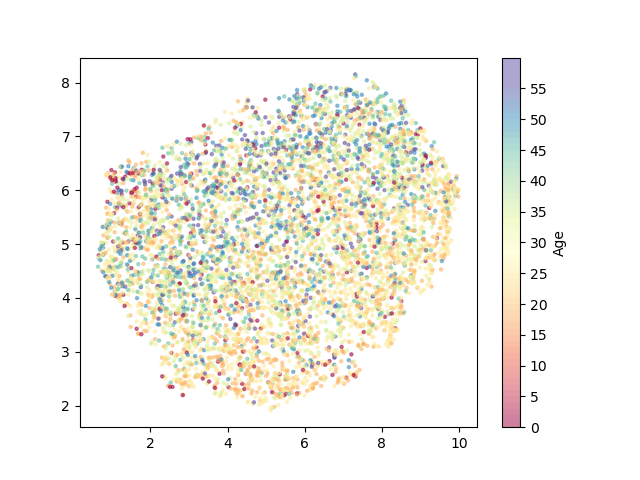
\includegraphics[width=\textwidth]{fig/umap_age.png}
        \caption{UMAP with label "Age"}
    \end{subfigure}
    \begin{subfigure}{0.49\textwidth}
        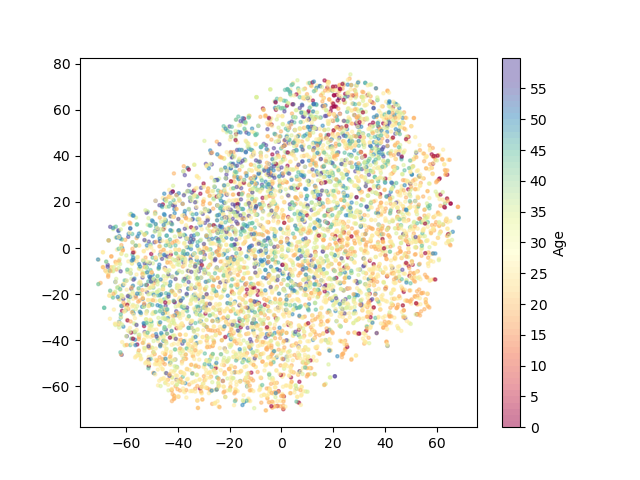
\includegraphics[width=\textwidth]{fig/tsne_age.png}
        \caption{t-SNE with label "Age"}
    \end{subfigure}
    \caption{Visualization of users' features}
    \label{fig:1}
\end{figure}

\subsection{Visualization of Movies' Features}
Similarly, we find out that the label "Genres" has better effect on clustering. We also count the frequencies of every single theme in "Genres". It turns out that Genres with smaller numbers in warm colors and those with larger numbers in cool colors do have different distributions of themes.
\begin{figure}[!ht]
    \centering
    \begin{subfigure}{0.49\textwidth}
        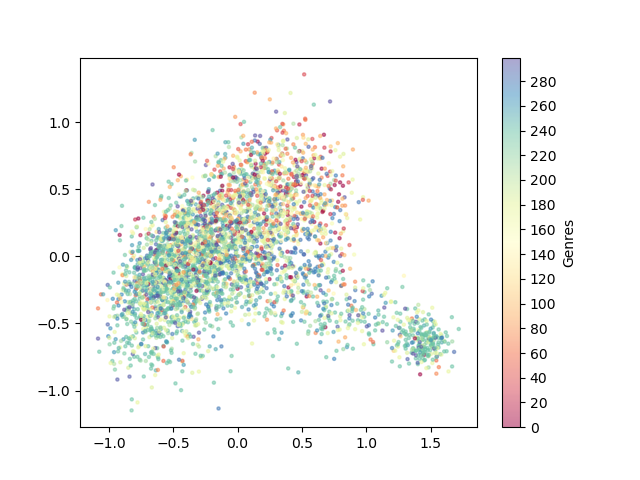
\includegraphics[width=\textwidth]{fig/pca_genres.png}
        \caption{PCA with label "Genres"}
    \end{subfigure}
    \begin{subfigure}{0.49\textwidth}
        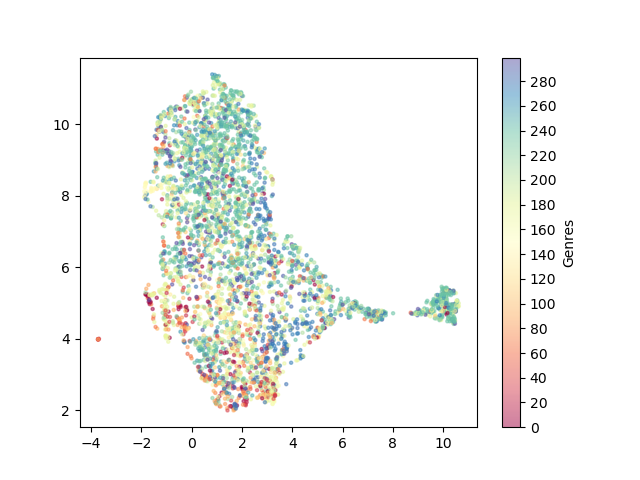
\includegraphics[width=\textwidth]{fig/umap_genres.png}
        \caption{UMAP with label "Genres"}
    \end{subfigure}
    \caption{Visualization of movies' features}
    \label{fig:2}
\end{figure}

\begin{figure}[!ht]
    \centering
    \begin{subfigure}{0.45\textwidth}
        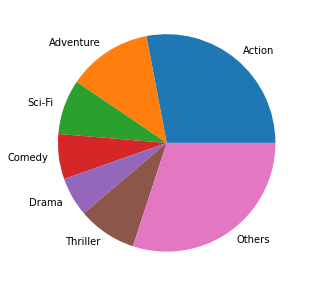
\includegraphics[width=0.9\textwidth]{fig/small_pie.png}
        \caption{First 100 genres}
    \end{subfigure}
    \begin{subfigure}{0.45\textwidth}
        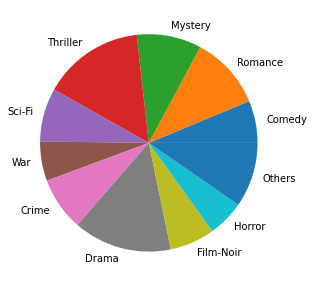
\includegraphics[width=0.9\textwidth]{fig/large_pie.png}
        \caption{Last 100 genres}
    \end{subfigure}
    \caption{Genres distributions}
\end{figure}

\newpage
\section{Contributions}
\begin{table}[ht]
    \begin{tabular}{ll}
        \textbf{Name} & \textbf{Tasks}\\
        Shuang Fan & Task 1.1 code, Task 1.1 report\\
        Kaiteng Jiang & Task 1.2 code, Task 1.2 report, Task 2 code, Task 2 report\\
        Shupei Li & Task 1.3 code, Task 1.3 report\\
    \end{tabular}
\end{table}
\vspace{2cm}
\section*{Appendix: Complete Results of Data Visualization}
\begin{figure}[H]
    \centering
    \begin{subfigure}{0.49\textwidth}
        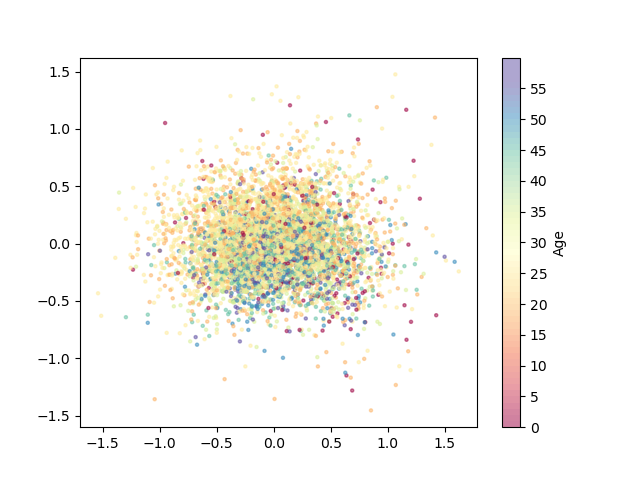
\includegraphics[width=\textwidth]{fig/pca_age.png}
        \caption*{(a) PCA with "Age"}
    \end{subfigure}
    \begin{subfigure}{0.49\textwidth}
        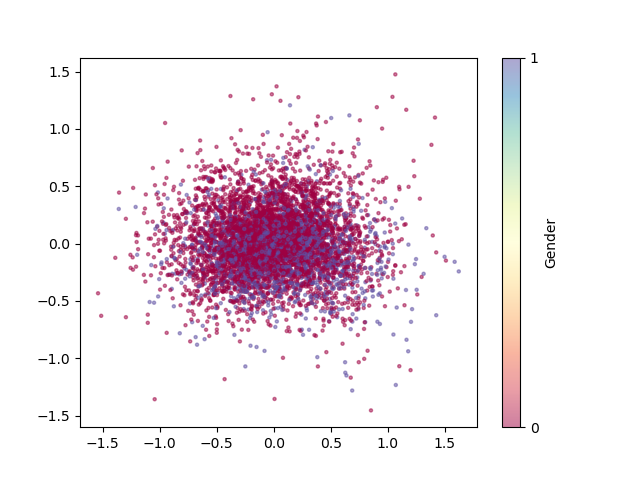
\includegraphics[width=\textwidth]{fig/pca_gender.png}
        \caption*{(b) PCA with "Gender"}
    \end{subfigure}
\end{figure}

\begin{figure}[H]
    \begin{subfigure}{0.49\textwidth}
        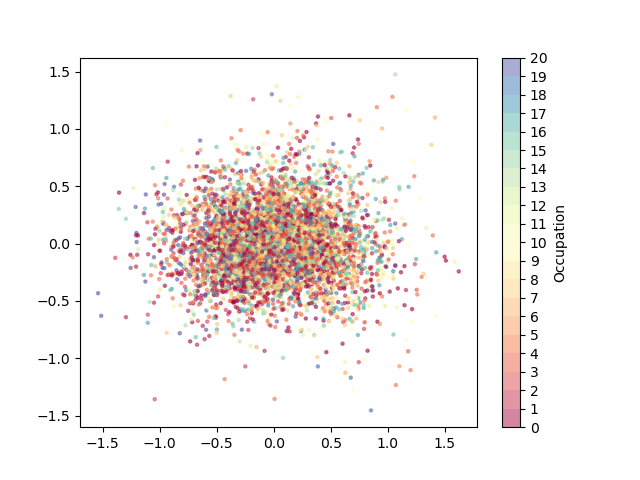
\includegraphics[width=\textwidth]{fig/pca_occ.png}
        \caption*{(c) PCA with "Occupation"}
    \end{subfigure}
    \begin{subfigure}{0.49\textwidth}
        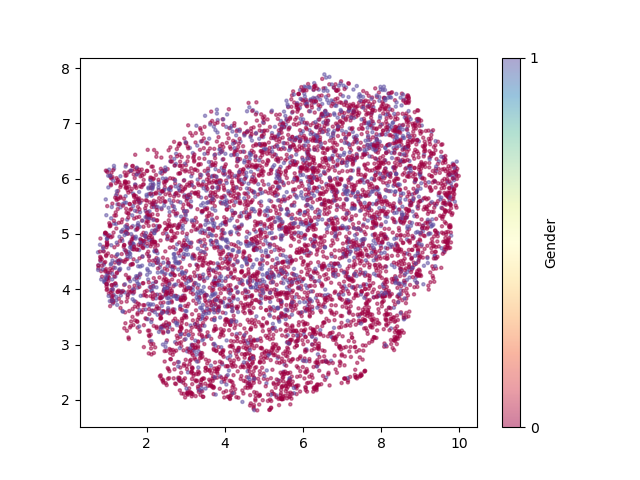
\includegraphics[width=\textwidth]{fig/umap_gender.png}
        \caption*{(d) UMAP with "Gender"}
    \end{subfigure}
    \begin{subfigure}{0.49\textwidth}
        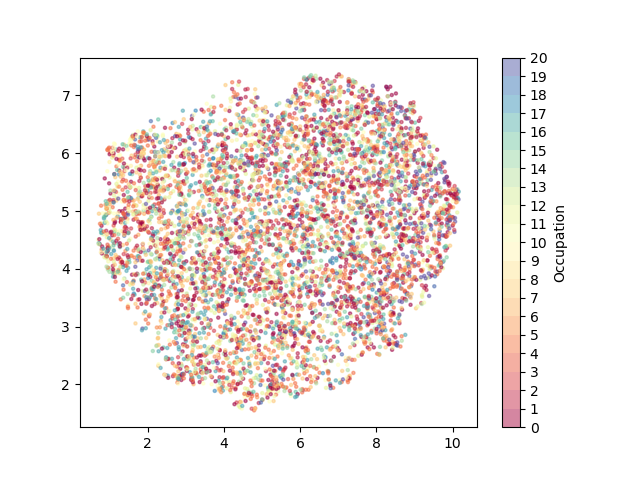
\includegraphics[width=\textwidth]{fig/umap_occ.png}
        \caption*{(e) UMAP with "Occupation"}
    \end{subfigure}
    \begin{subfigure}{0.49\textwidth}
        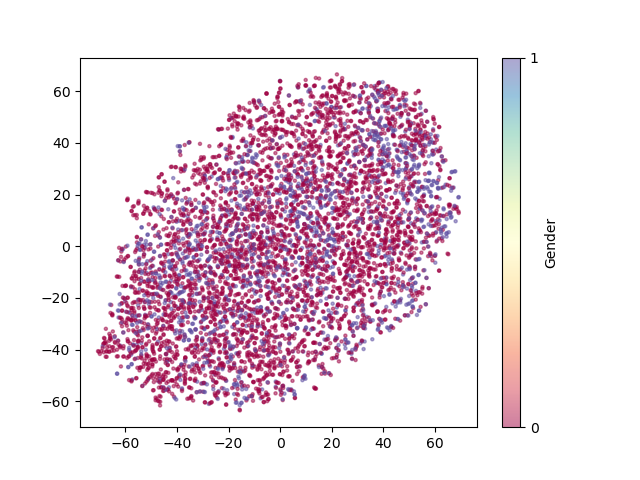
\includegraphics[width=\textwidth]{fig/tsne_gender.png}
        \caption*{(f) t-SNE with "Gender"}
    \end{subfigure}
    \begin{subfigure}{0.49\textwidth}
        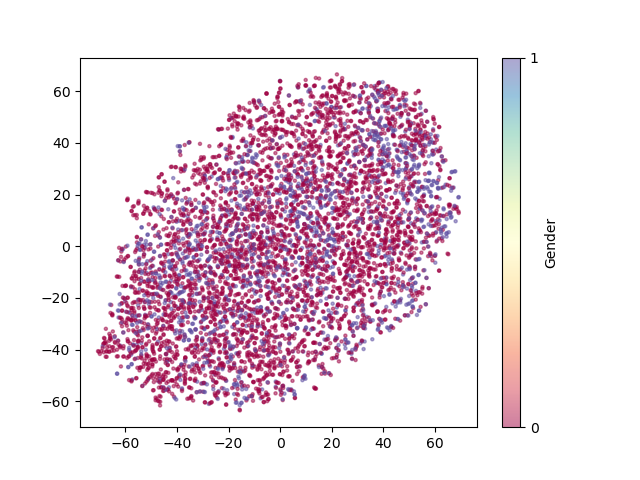
\includegraphics[width=\textwidth]{fig/tsne_gender.png}
        \caption*{(g) t-SNE with "Gender"}
    \end{subfigure}
    \caption{Visualization of users' features}
\end{figure}

\newpage

\begin{figure}[H]
    \centering
    \begin{subfigure}{0.49\textwidth}
        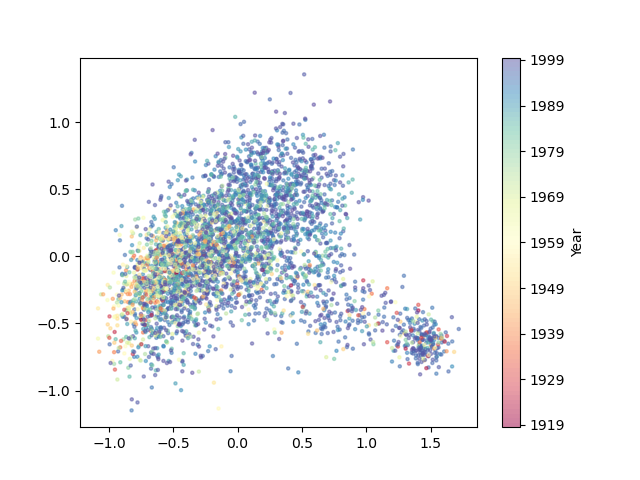
\includegraphics[width=\textwidth]{fig/pca_year.png}
        \caption{PCA with "Year"}
    \end{subfigure}
    \begin{subfigure}{0.49\textwidth}
        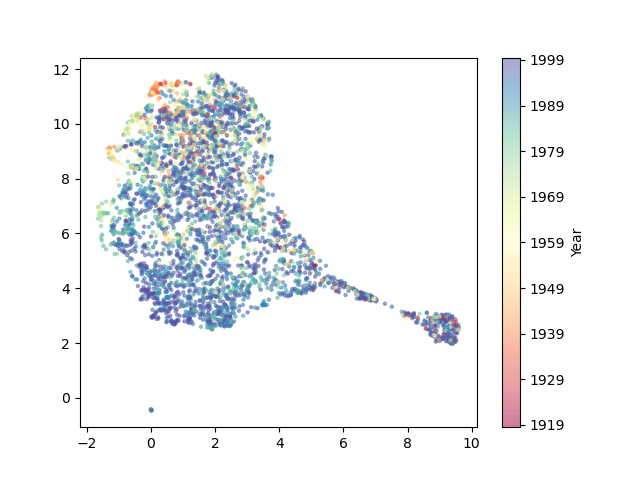
\includegraphics[width=\textwidth]{fig/umap_year.png}
        \caption{UMAP with "Year"}
    \end{subfigure}

    \begin{subfigure}{0.49\textwidth}
        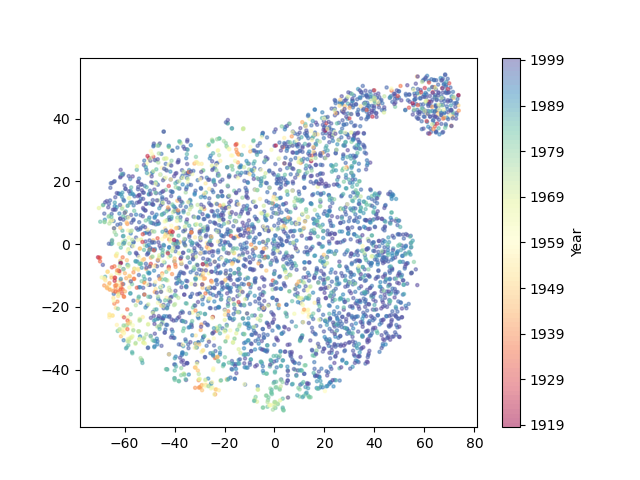
\includegraphics[width=\textwidth]{fig/tsne_year.png}
        \caption{t-SNE with "Year"}
    \end{subfigure}
    \begin{subfigure}{0.49\textwidth}
        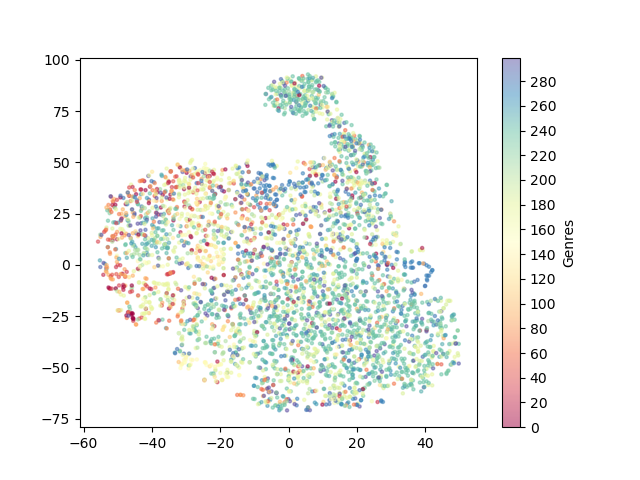
\includegraphics[width=\textwidth]{fig/tsne_genres.png}
        \caption{t-SNE with "Genres"}
    \end{subfigure}
    \caption{Visualization of movies' features}
\end{figure}

\end{document}
